\documentclass[a4paper]{article}

\usepackage[utf8]{inputenc}
\usepackage[authoryear,round]{natbib}
\usepackage{graphicx}
\usepackage{hyperref}
\usepackage{url}
\usepackage{a4wide}
\usepackage [ table ]{ xcolor }
\usepackage{color}
\usepackage{amssymb,amsmath}
\usepackage{amsfonts}
\usepackage{graphicx} 
\usepackage{braket}
\usepackage{listings}
\sloppy

\newcommand{\RFORGE}{R-Forge Administration and Development Team}

\title{R-Forge Installation and Administration Manual, ALPHA}
\author{\RFORGE}
\date{\today}


\let\code=\texttt
\let\email=\texttt
\newcommand{\pkg}[1]{{\normalfont\fontseries{b}\selectfont #1}}
\newcommand{\proglang}[1]{\textsf{#1}}
\newcommand{\class}[1]{`\code{#1}'}

\begin{document}

\pagestyle{empty} 

\begin{titlepage}

  {\LARGE \raggedleft \textbf{R-Forge Installation and Administration Manual, {\large ALPHA}}}\\
%%  \vspace*{0.5cm}
  \rule{\linewidth}{1.5mm}
  \begin{flushright}
  \textbf{SVN Revision: xx, \today}\\
  \end{flushright}

  \vspace*{\fill}
%%  \vspace*{10cm} 
   
  {\Large
    \noindent {\textbf{\RFORGE{}}\\
    \rule{\linewidth}{1mm}} 
  }
  
\end{titlepage}


\newpage
\vspace*{\fill}

%% Copyright notices
%%\noindent Copyright 2006--2007 Stefan Theussl\\
\noindent Copyright 2006--2008 \RFORGE{}\\

\vspace{0.5cm}
%
\includegraphics{CCAL.png} 
\vspace{1cm}

\noindent The content in this manual is licensed
under a Creative Commons Attribution-Share Alike 2.0 license. 

\vspace{0.5cm}
The \RFORGE{} has chosen to apply the Creative
Commons Attribution License (CCAL) to this manual, i.e., that under the CCAL,
the authors retain ownership of the copyright 
for this manual, but the authors allow anyone to download, reuse,
reprint, modify, distribute, and/or copy the contents of this manual,
so long as the original authors and source are 
credited. Furthermore, the authors permit others to distribute
derivative works only under the same license or one compatible with
the one that governs the authors' work. 
This broad license was developed to facilitate open access
to, and free use of, original works of all types. Applying this
standard license to this work will ensure the authors' right to make
this work freely and openly available (see
\url{http://creativecommons.org/licenses/by-sa/2.0/} for details). 

\vspace{0.5cm}
The current members of the \RFORGE{} are Kurt Hornik, Martin Kober,
David Meyer, Stefan Theu\ss{}l and Achim Zeileis. To contact the
authors please write an email to \email{R-Forge@R-project.org}.

\newpage

\pagenumbering{roman}
\pagestyle{plain}
\tableofcontents

\clearpage
\pagestyle{headings}
\pagenumbering{arabic}
\setcounter{page}{1}

\section{Introduction}

Operating System Debian, reference to Rnews Article
R-Forge~User's~Manual

Subversion~\citep[SVN,
see][]{forge:Pilato+Collins-Sussman+Fitzpatrick:2004} or Concurrent
Versions System~\citep[CVS, see][]{forge:Cederqvist:2006}


\newpage
\section{Installation}
\label{sec:installation}

\subsection{Setup basis Debian Instance}

Before start working with the FusionForge, please install Virtual Machine using the latest
Debian stable Distribution. 

\vspace{0.5cm}
We use Xen virtualization infrastructure:

\begin{itemize}
	\item xsrforge.wu.ac.at: Xen Server (dom0)
	\item r-forge.wu.ac.at: R-Forge live instance (xmrforge2)
	\item r-forge-devel.wu.ac.at: R-Forge devel instance (xmrforge1)
\end{itemize}

\subsection{FusionForge}

The installation instruction describes setting up the R-Forge ``devel'' instance.

A backup of the base Debian system is created as an 
LVM snapshot (xmrforge1-disk-snapshot).

\begin{enumerate}
	\item Systemconfiguration:
	
hostname: xmrforge1 (already done.)
\par Debian flavor: Lenny
	

add the following entries:	
CRAN Debian Packages
\par
\medskip
\definecolor{light-gray}{gray}{0.95}	
\fboxrule=0.2mm
\noindent \fcolorbox{black}{light-gray}{\code {echo "deb
    http://cran.r-project.org/bin/linux/debian lenny-cran/"  /etc/apt/sources.list}}
\medskip

FusionForge packages
\medskip
\definecolor{light-gray}{gray}{0.95}	
\fboxrule=0.2mm

\noindent \fcolorbox{black}{light-gray}{\verb{echo"deb
    http://fusionforge.fusionforge.org/debian lenny main/" /etc/apt/sources.list}}
\medskip

Add key information (optional (if the retrieval of third - party keys
is reqested, do the following:

\medskip
\definecolor{light-gray}{gray}{0.95}	
\fboxrule=0.2mm
\noindent \fcolorbox{black}{light-gray}{\code{#gpg --recv-keys 06F90DE5381BA480}}
\medskip

\medskip
\definecolor{light-gray}{gray}{0.95}	
\fboxrule=0.2mm
\noindent \fcolorbox{black}{light-gray}
{\code{# gpg --export --armor 06F90DE5381BA480 | sudo apt-key add -}}
\medskip
	

	\item Install base packages

\medskip
\definecolor{light-gray}{gray}{0.95}	
\fboxrule=0.2mm
\noindent \fcolorbox{black}{light-gray}{\code{# aptitude install subversion joe emacs ess r-base r-recommended bzip rsync less}}
\medskip

	\item Checkout radmin

\medskip
\definecolor{light-gray}{gray}{0.95}	
\fboxrule=0.2mm
\noindent \fcolorbox{black}{light-gray}{\code{\$ mkdir svn}}
\par \noindent \fcolorbox{black}{light-gray}{\code{\$ cd svn}}
\par \noindent \fcolorbox{black}{light-gray}{\code{\$ svn co svn://svn-statmath.wu.ac.at/radmin radmin}}
\medskip


\item configure ssh daemon 

copy sshd\_config from radmin repository

\item configure rsync daemon 

copy rsyncd.conf from radmin repository and add line to inetd.conf

Optional * homeverzeichnis nach /srv linken

\end{enumerate}


\section{Components}
\label{sec:registration}

\subsection{Filesystem}

Filesystem on R-Forge 

o File System Information (Xen Server)
		Filesystem            Size  Used Avail Use% Mounted on
		/dev/sda2              76G  7.1G   65G  10% /
		tmpfs                 5.9G     0  5.9G   0% /lib/init/rw
		udev                   10M   52K   10M   1% /dev
		tmpfs                 5.9G     0  5.9G   0% /dev/shm

	o Volume Group Information:
\begin{lstlisting}
  --- Volume group ---
  VG Name               vgforge0
  System ID             
  Format                lvm2
  Metadata Areas        1
  Metadata Sequence No  31
  VG Access             read/write
  VG Status             resizable
  MAX LV                0
  Cur LV                10
  Open LV               7
  Max PV                0
  Cur PV                1
  Act PV                1
  VG Size               1.27 TB
  PE Size               4.00 MB
  Total PE              333754
  Alloc PE / Size       252672 / 987.00 GB
  Free  PE / Size       81082 / 316.73 GB
  VG UUID               Ol5cqb-YFyz-4Mk0-UC1f-Mbmc-TkE0-NlJG0N

	o Logical Volumes Information:
xsrforge:/home/theussl/svn/radmin/Install-Notes# lvdisplay
  --- Logical volume ---
  LV Name                /dev/vgforge0/xmrforge-srvdisk
  VG Name                vgforge0
  LV UUID                GYiAxS-zBrs-0IdV-Fedj-gLLV-ZGJY-SbyqyC
  LV Write Access        read/write
  LV Status              available
  # open                 1
  LV Size                530.00 GB
  Current LE             135680
  Segments               2
  Allocation             inherit
  Read ahead sectors     0
  Block device           253:2
   
  --- Logical volume ---
  LV Name                /dev/vgforge0/xmorthanc-disk
  VG Name                vgforge0
  LV UUID                6UO4Aa-MXta-C4fZ-az7f-gH1o-Bp6P-WZKKlp
  LV Write Access        read/write
  LV Status              available
  # open                 1
  LV Size                200.00 GB
  Current LE             51200
  Segments               2
  Allocation             inherit
  Read ahead sectors     0
  Block device           253:3
   
  --- Logical volume ---
  LV Name                /dev/vgforge0/xmorthanc-swap
  VG Name                vgforge0
  LV UUID                u6zLwO-6sG8-2G1T-iHrF-Go0N-Nuav-EYXAyG
  LV Write Access        read/write
  LV Status              available
  # open                 1
  LV Size                1.00 GB
  Current LE             256
  Segments               1
  Allocation             inherit
  Read ahead sectors     0
  Block device           253:4
   
  --- Logical volume ---
  LV Name                /dev/vgforge0/xmrforge2-disk
  VG Name                vgforge0
  LV UUID                WNunp0-oG94-llIw-Msuy-BRQt-ro2e-2sXmKp
  LV Write Access        read/write
  LV Status              available
  # open                 1
  LV Size                10.00 GB
  Current LE             2560
  Segments               1
  Allocation             inherit
  Read ahead sectors     0
  Block device           253:7
   
  --- Logical volume ---
  LV Name                /dev/vgforge0/xmrforge2-swap
  VG Name                vgforge0
  LV UUID                Eqf2RV-GTAJ-x3pS-Ekbs-5UFz-bzHl-1rmFHm
  LV Write Access        read/write
  LV Status              available
  # open                 1
  LV Size                2.00 GB
  Current LE             512
  Segments               1
  Allocation             inherit
  Read ahead sectors     0
  Block device           253:8
   
  --- Logical volume ---
  LV Name                /dev/vgforge0/xmcran-disk
  VG Name                vgforge0
  LV UUID                wtnV22-NWBg-xqpA-FVtd-GyBX-rPcK-EQl1vP
  LV Write Access        read/write
  LV Status              available
  # open                 0
  LV Size                10.00 GB
  Current LE             2560
  Segments               1
  Allocation             inherit
  Read ahead sectors     0
  Block device           253:10
   
  --- Logical volume ---
  LV Name                /dev/vgforge0/xmcran-swap
  VG Name                vgforge0
  LV UUID                Slglg3-D8y7-xrjv-5Uzw-leA2-l83R-ZBXndU
  LV Write Access        read/write
  LV Status              available
  # open                 0
  LV Size                2.00 GB
  Current LE             512
  Segments               1
  Allocation             inherit
  Read ahead sectors     0
  Block device           253:11
   
  --- Logical volume ---
  LV Name                /dev/vgforge0/xmcran-srvdisk
  VG Name                vgforge0
  LV UUID                7mOBmE-AHzY-mNhd-OBMc-VVRf-6Vzd-Ri60rl
  LV Write Access        read/write
  LV Status              available
  # open                 0
  LV Size                200.00 GB
  Current LE             51200
  Segments               1
  Allocation             inherit
  Read ahead sectors     0
  Block device           253:12
   
  --- Logical volume ---
  LV Name                /dev/vgforge0/xmrforge1-disk
  VG Name                vgforge0
  LV UUID                YYUVax-5sTP-0tRY-dtud-2c6I-h5Qk-HXqz2c
  LV Write Access        read/write
  LV Status              available
  # open                 1
  LV Size                30.00 GB
  Current LE             7680
  Segments               1
  Allocation             inherit
  Read ahead sectors     0
  Block device           253:13
   
  --- Logical volume ---
  LV Name                /dev/vgforge0/xmrforge1-swap
  VG Name                vgforge0
  LV UUID                whqc2X-QTQG-aqFS-V0Pd-RV4M-pQjh-Nupqik
  LV Write Access        read/write
  LV Status              available
  # open                 1
  LV Size                2.00 GB
  Current LE             512
  Segments               1
  Allocation             inherit
  Read ahead sectors     0
  Block device           253:14
\end{lstlisting}

\subsection{Serverfarm---map}

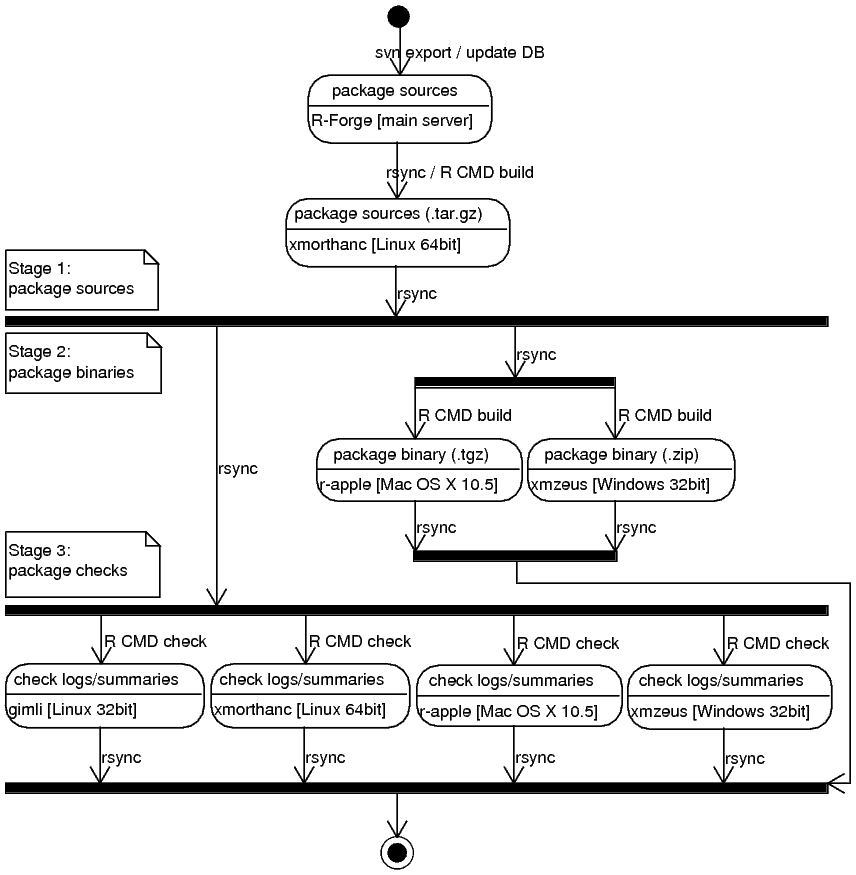
\includegraphics[width=15cm]{Rbuild}

\subsection{GForge}

GForge is an open source software originally created for the
SourceForge. GForge has a GNU license and provides project hosting,
version control, bug-tracking, and messagign.

Install FusionForge base system

\medskip
\definecolor{light-gray}{gray}{0.95}	
\fboxrule=0.2mm
\noindent \fcolorbox{black}{light-gray}{\code{aptitude install gforge gforge-plugin-scmsvn gforge-mta-postfix postfix}}
\medskip

\par
Further configuration: 
postfix: Internet site 
mailman: Missing site list 

Mailman needs a so-called "site list", which is the list from
which password reminders and such are sent out from.  This list
needs to be created before mailman will start. To create
the list, run "newlist mailman" and follow the instructions on-screen.
Note that you also need to start mailman after that, using
/etc/init.d/mailman start.

GForge administrator password: \textless some password\textgreater


proFTP: from inetd

changed config files: postfix/main.cf, postfix/aliases, etc/nsswitch.conf, proftp.conf

Further installation: 

\medskip
\definecolor{light-gray}{gray}{0.95}	
\fboxrule=0.2mm
\noindent \fcolorbox{black}{light-gray}{\code{apt-get install postgresql-contrib gforge-plugin-mediawiki}}
\medskip


\subsubsection{GForge setup}

\medskip
\definecolor{light-gray}{gray}{0.95}	
\fboxrule=0.2mm
\noindent \fcolorbox{black}{light-gray}{\code{apt-get install gforge}}
\medskip

If the installation process breaks, do the following:
\begin{enumerate}
\item copy ssl keys
cp -r /home/theussl/r-forge.bak/etc/apache2/ssl /etc/apache2/ssl
\item edit gforge.conf and insert the location of the ssl certificate and key
vi /etc/gforge/gforge.conf
\item 
\begin{lstlisting} tell postgresql to listen on tcp sockets (tcpip_socket = true)
vi /etc/postgresql/7.4/main/postgresql.conf
/etc/init.d/postgresql-7.4 restart
\end{lstlisting}

\item continue with 
\medskip
\definecolor{light-gray}{gray}{0.95}	
\fboxrule=0.2mm
\noindent \fcolorbox{black}{light-gray}{\code{apt-get install gforge}}
\medskip

\item afterwards: change /etc/gforge/gforge.conf and run
gforge-config
\item furthermore you have to uncomment extension=pgsql.so:
vi /etc/php4/apache2/php.ini

\item install svn plugin
\medskip
\definecolor{light-gray}{gray}{0.95}	
\fboxrule=0.2mm
\noindent \fcolorbox{black}{light-gray}{\code{apt-get install gforge-plugin-scmsvn}}
\medskip

\item \begin{lstlisting}replace /usr/lib/gforge/plugins/scmsvn/bin/svn_update.pl with the script from radmin rep
\item copy svnsetup.sh from radmin rep to /usr/local/bin/
\item verify that the svnbasedir repository exists in /svnroot/
\end{lstlisting}

\item link gforge www dir to /srv
cd /usr/share/gforge
\begin{lstlisting}R-Forge:/usr/share/gforge# mv www www.old
R-Forge:/usr/share/gforge# ln -s /srv/www/ www

\item FIXME /svnroot should point to /srv/svn
ln -s /var/lib/gforge/chroot/svnroot/ /svnroot


r-forge:/home/theussl# /usr/lib/mailman/bin/newlist mailman

\item make changes according to manual
emacs /usr/lib/mailman/Mailman/mm_cfg.py
\end{lstlisting}
\end{enumerate}

The following steps have to be done after installation and each update
\begin{lstlisting}
Setup gforge scripts accordingly (gforge-scripts@r-forge-root)
- SVN: dumps predefined structure in fresh repositories
- SSH-KEYS: deny shell login, port forwarding etc. in gforge ssh key creation
- VIEW-CVS: change location of viewcvs script accordingly

Further changes made to gforge

- copy favicon from svn to /srv/www/
- copy Base.tab from svn to /srv/www/include/languages/Base.tab
- uncomment Top Project Download lines in /srv/www/include/features_boxes.php 

svn-commit statistics don't work

- Bugged index, probably fixed in newer versions
- connect to db gforge
- DROP INDEX statscvsgrp_oid;
- (Index was: '"statscvsgrp_oid" UNIQUE, btree ("month", "day")')


Setting up plugin_rforge in the DB

- create the table

CREATE TABLE plugin_rforge_package_db (
    pkg_name character varying(255) NOT NULL PRIMARY KEY,
    unix_group_name character varying(30) NOT NULL,
    version character varying(30),
    title text,
    description text,
    author text,
    license text,
    pkg_date date,
    last_change timestamp with time zone,
    rev integer
);
CREATE INDEX plugin_rforge_package_db_unixgn ON plugin_rforge_package_db (unix_group_name);


- create user with rights in the table
    CREATE user plugin_rforge password 'jenslf0r2';
    GRANT all on plugin_rforge_package_db to plugin_rforge;
\end{lstlisting}
\par More under \url{http://gforge.org/gf}

\subsection{Postfix}
Postfix is an open source mail transfer agent requires that the file system can rename a file to a near-by
directory without changing the file's inode number.

For more details about Postfix visit \url{http://www.postfix.org/}

\subsection{Subversion}

Subverion is a version control system used to maintain current and
historical versions of files and source code as well as web pages and
documentation.
\par More about SVN under \url{http://subversion.tigris.org/}

\subsection{Mailman}
Mailman needs a so-called "site list", which is the list from
which password reminders and such are sent out from.  This list
needs to be created before mailman will start. To create
the list, run "newlist mailman" and follow the instructions on-screen.
Note that you also need to start mailman after that, using
\code{/etc/init.d/mailman} start.

GForge administrator password: <some password>

proFTP: from inetd

changed config files: postfix/main.cf, postfix/aliases, etc/nsswitch.conf, proftp.conf
\par
Further installation: 
\par \definecolor{light-gray}{gray}{0.95}
\fboxrule=0.2mm
\noindent \fcolorbox{black}{light-gray}{\code{apt-get install postgresql-contrib gforge-plugin-mediawiki}}
\medskip

\subsection{\proglang{R} - Installation}

\medskip
\definecolor{light-gray}{gray}{0.95}	
\fboxrule=0.2mm
\noindent \fcolorbox{black}{light-gray}{\code{apt-get install r-base r-recommended}}
\medskip

\medskip
\definecolor{light-gray}{gray}{0.95}	
\fboxrule=0.2mm
\noindent \fcolorbox{black}{light-gray}{\code{apt-get install rsync}}
\medskip


* check results:
* rsync-daemon - eintrag in /etc/inetd.conf

rsync           stream tcp nowait root /usr/bin/rsync rsyncd --daemon

* erstelle rsync.conf

uid = nobody
gid = nogroup

[R.check]
        path = /srv/rsync/R.check
        comment = CRAN daily check results
\begin{lstlisting}
r-forge:/home# chmod 664 /etc/rsyncd.conf
r-forge:/home# chgrp cranadmin /etc/rsyncd.conf
\end{lstlisting}

\subsection{CRAN public rsync}


WARNING: change get-Rpub.sh so that it points to the right directory
cp /home/theussl/svn/radmin/R-forge-root/etc/cron.d/getRpub /etc/cron.d/getRpub
cp /home/theussl/svn/radmin/R-forge-root/usr/local/bin/get-Rpub.
sh /usr/local/bin/
chmod 775 /usr/local/bin/get-Rpub.sh
chown root.cranadmin /usr/local/bin/get-Rpub.sh

\medskip
\definecolor{light-gray}{gray}{0.95}	
\fboxrule=0.2mm
\noindent \fcolorbox{black}{light-gray}{\code{mkdir /srv/R/}}
\medskip
\par
\medskip
\definecolor{light-gray}{gray}{0.95}	
\fboxrule=0.2mm
\noindent \fcolorbox{black}{light-gray}{\code{mkdir /srv/R/CRAN}}
\medskip
\par
\medskip
\definecolor{light-gray}{gray}{0.95}	
\fboxrule=0.2mm
\noindent \fcolorbox{black}{light-gray}{\code{chmod -R 2775 /srv/R}}
\medskip


touch /var/log/rsync.log
chown root.cranadmin /var/log/rsync.log
chmod 664 /var/log/rsync.log

get-Rpub.sh

Bioconductor mirror
cronjob

\medskip
\definecolor{light-gray}{gray}{0.95}	
\fboxrule=0.2mm
\noindent \fcolorbox{black}{light-gray}{\code{cp /home/theussl/svn/radmin/R-forge-root/etc/cron.daily/bioc /etc/cron.daily/}}
\medskip

Copy download script

\medskip
\definecolor{light-gray}{gray}{0.95}	
\fboxrule=0.2mm
\noindent \fcolorbox{black}{light-gray}{\code{cp
    /home/theussl/svn/radmin/R-forge-root/usr/local/bin/bioc.sh
    /usr/local/bin/}}
\noindent \fcolorbox{black}{light-gray}{\code{chown root.cranadmin /usr/local/bin/bioc.sh}}
\par \noindent \fcolorbox{black}{light-gray} {\code{chmod 775 /usr/local/bin/bioc.sh}}\medskip

Firewall: port open

\subsection{Install java}

\medskip
\definecolor{light-gray}{gray}{0.95}	
\fboxrule=0.2mm
\noindent \fcolorbox{black}{light-gray}{\code{edit /etc/apt/sources.list}}
\medskip


For sun-java5 packages in unstable
deb http://ftp.at.debian.org/debian/ sid non-free
deb-src http://ftp.at.debian.org/debian/ sid non-free

Edit /etc/apt/apt.conf
// set the default release to etch
APT::Default-Release "etch";

\medskip
\definecolor{light-gray}{gray}{0.95}	
\fboxrule=0.2mm
\noindent \fcolorbox{black}{light-gray}{\code{apt-get -t unstable install sun-java6-jdk sun-java6-jre}}
\medskip


Use vim as default editor
update-alternatives --config editor



\section{Release and Quality Management System}
\label{sec:release_and_QM}

\subsection{Serverfarm}
\subsection{Mac OSX}
\subsection{Linux}
\subsection{Windows}

%% Acknowledgements from Rnews article
\section{Acknowledgements}

Setting up this project would not have been possible without Douglas
Bates and the University of Wisconsin as they provided us with a
server for hosting this platform. Furthermore, 
the authors would like to thank the Zentrum f\"ur Informatikdienste  
of the Wirtschaftsuniversit\"at Wien for
their support and for providing us with additional hardware as well as a
professional server infrastructure. 
Thanks to Philippe Grosjean for
providing a Mac~OS description (Section~\ref{sec:scm-macosx}).

\bibliographystyle{plainnat}
\bibliography{R-Forge_Manual}
\end{document}
